% % % % % % % % % % % % % % % % % % % % % % % % % % % % % % % % % % % % % % % % % % % %
%                                                                                     %
% Short Sectioned Assignment LaTeX Template Version 1.0 (5/5/12)                      %
% This template has been downloaded from: http://www.LaTeXTemplates.com               %
%                                                                                     %
% Original author:  Frits Wenneker (http://www.howtotex.com)                          %
%                                                                                     %
% Modified by: Fco Javier Sueza Rodríguez (fcosueza@disroot.org)                      %
%                                                                                     %
% Changes:                                                                            %
%           - Document type scrarticle                                                %
%           - Use babel-lang-spanish package and marvosym                             %
%           - Use hyperref, enumitem and tcolorbox                                    %
%           - Use fancyhdr package an configure it                                    %
%           - Use Time New Roman (mathptmx), Helvetic and Courier fonts               %
%                                                                                     %
% License: CC BY-NC-SA 3.0 (http://creativecommons.org/licenses/by-nc-sa/3.0/)        %
%                                                                                     %
% % % % % % % % % % % % % % % % % % % % % % % % % % % % % % % % % % % % % % % % % % % %

%-----------------------------------------------%
%	              Packages                  %
%-----------------------------------------------%

\documentclass[bibliography=totoc]{scrarticle}

% ---- Text Input/Output ----- %

\usepackage[T1]{fontenc}
\usepackage[utf8]{inputenc}
\usepackage{mathptmx}
\usepackage[scaled=.92]{helvet}
\usepackage{courier}
\usepackage[indent=12pt]{parskip}
\usepackage[titletoc, title]{appendix}

\usepackage{geometry}
\geometry{verbose,tmargin=3cm,bmargin=3cm,lmargin=2.5cm,rmargin=2.5cm}

% ---- Language ----- %

\usepackage[spanish, es-tabla, es-noquoting]{babel}
\usepackage{marvosym}

% ---- Another packages ---- %

\usepackage[toc, sort=use]{glossaries}
\usepackage{amsmath,amsfonts,amsthm}
\usepackage{graphics,graphicx}
\usepackage{tcolorbox}
\usepackage{hyperref}
\usepackage{enumitem}
\usepackage{fancyhdr}
\usepackage{float}
\usepackage{ulem}


%--------------------------------------------------------------------%
%                      Customizing Document                          %
%--------------------------------------------------------------------%

% -------------- Customize headers and footers---------------------- %

\pagestyle{fancy}

\fancyhead[]{}
\fancyfoot[L]{}
\fancyfoot[C]{}
\fancyfoot[R]{\thepage}

\renewcommand{\headrulewidth}{0pt} % Remove header underlines
\renewcommand{\footrulewidth}{0pt} % Remove footer underlines

% Needed to get first page footer correctly
\fancypagestyle{plain}{
    \fancyhf{}
    \fancyfoot[R]{\thepage}
}

% --------------------- Packages Configuration --------------------- %


\hypersetup{
    colorlinks=true,
    linkcolor=magenta,
    urlcolor=magenta
}

\setcounter{secnumdepth}{4}
\setcounter{tocdepth}{4}
\graphicspath{{./images/}}

\setlength{\headheight}{13.6pt} % Customize the height of the header
\numberwithin{figure}{section} % Number figures within sections
\numberwithin{table}{section}

% ------------------------ New Commands ----------------------------- %

\newcommand{\horrule}[1]{\rule{\linewidth}{#1}} % Create horizontal rule command

% ------------------------ Anexx now with name in spanish before title ----------------------- %

\addto\captionsspanish{%
	\renewcommand\appendixname{Anexo}
	\renewcommand\appendixpagename{Anexos}
}




%----------------------------------------------------------------------------------------
%	TÍTULO Y DATOS DEL ALUMNO
%----------------------------------------------------------------------------------------

\title{
\vspace{10ex}
\normalfont \normalsize
\huge \textbf{Conociendo los Modelos de Inteligencia Artificial}
}
\author{Francisco Javier Sueza Rodríguez}
\date{\normalsize\today}

\glsenablehyper
\makeglossaries
\loadglsentries{glos}

%----------------------------------------------------------------------------------------
%                                     DOCUMENTO
%----------------------------------------------------------------------------------------
\begin{document}


\maketitle

\thispagestyle{empty}

\vspace{75ex}

\begin{center}
    \begin{tabular}{l l}
        \textbf{Centro}: & IES Zaidin-Vergeles \\
        \textbf{Curso}: & Inteligencia Artificial y Big Data\\
        \textbf{Módulo}: & Modelos de Inteligencia Artificial \\
    \end{tabular}
\end{center}

\newpage

\begingroup
\hypersetup{linkcolor=black}
\tableofcontents
\endgroup

\newpage

\begingroup
\hypersetup{linkcolor=black}
\listoffigures             
\endgroup

\newpage

\section{Introducción}
En este documento se incluye la \textbf{Actividad de la unidad 1} de la asignatura de Modelos de Inteligencia Artificial. Tal y como recomendaba la profesora en una de las videoconferencias, se ha realizado finalmente en un único documento PDF, separando en cada sección las diferentes partes de las que se compone la actividad.

\section{Parte 1: Perspectivas de IA}
En esta parte se realizará un debate colaborativo y un informe del diseño individual de una IA.                                

\subsection{Debate en Foro: Clasificación y Análisis Crítico}
Se ha realizado una contribución al foro, dentro del hilo \textbf{Pensar Racionalmente} que es el que le ha tocado a mi subgrupo. Además, se ha realizado un comentario sobre la publicación de una compañera que había elegido el sistema experto DXPlain. Aunque se puede ver la contribución al debate en el foro, se incluyen capturas de estas, que vemos a continuación.

\begin{figure}[ht]
	\centering
	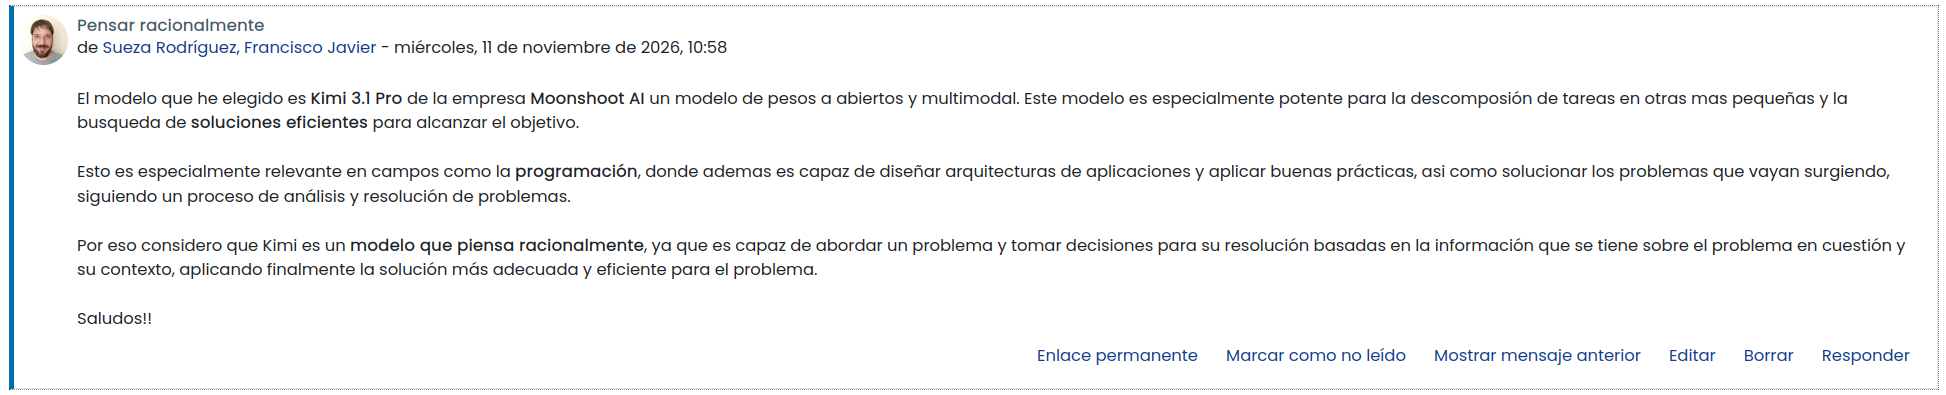
\includegraphics[scale=0.32]{foro.png}
	\caption{Creación de mensaje en el foro}
\end{figure}


\begin{figure}[ht]
	\centering
	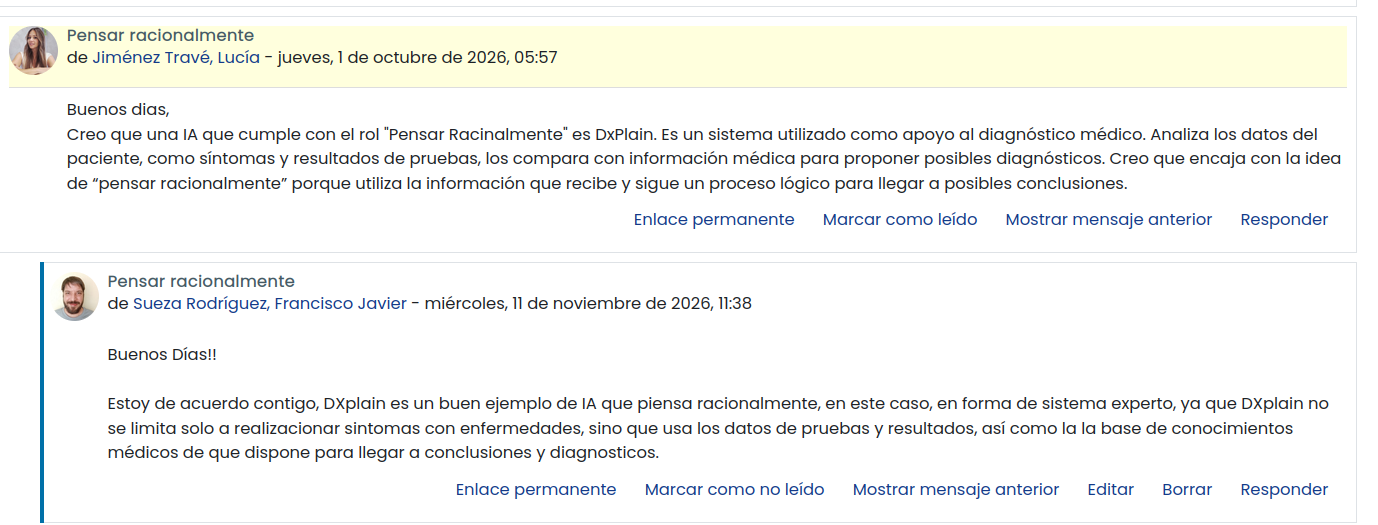
\includegraphics[scale=0.47]{foro-2.png}
	\caption{Replica al debate}
\end{figure}


\subsection{Informe Técnico}

\newpage

\bibliography{citas}
\bibliographystyle{unsrt}


\end{document}  